% CREATED BY DAVID FRISK, 2016
% MODIFIED BY JAKOB JARMAR, 2016
% A few changes by Birgit Grohe, 2017 and 2018
% Adjustments with the help of Gustav Örtenberg 2019
% Parskip % bibliography system updated by Erik Ljungdahl, May 2022

% IMPORT SETTINGS
\documentclass[12pt,a4paper,twoside,openright]{report}
% CREATED BY DAVID FRISK, 2016

% BASIC SETTINGS
\usepackage{moreverb}								% List settings
\usepackage{textcomp}								% Fonts, symbols etc.
\usepackage{lmodern}								% Latin modern font
\usepackage{helvet}									% Enables font switching
\usepackage[T1]{fontenc}							% Output settings
\usepackage[english]{babel}							% Language settings
\usepackage[utf8]{inputenc}							% Input settings
\usepackage{amsmath}								% Mathematical expressions (American mathematical society)
\usepackage{amssymb}								% Mathematical symbols (American mathematical society)
\usepackage[pdf]{graphviz}                          % dot-files directly in latex
\usepackage{graphicx}								% Figures
% \usepackage{subfig}									% Enables subfigures
\usepackage{caption}
\usepackage{subcaption}
\usepackage{acronym}                                % For a list of abbreviations
\usepackage{glossaries}
\usepackage{tikz-dependency}

\numberwithin{equation}{chapter}					% Numbering order for equations
\numberwithin{figure}{chapter}						% Numbering order for figures
\numberwithin{table}{chapter}						% Numbering order for tables
\usepackage{minted}					% Enables source code listings
\usepackage{chemfig}								% Chemical structures
\usepackage[top=3cm, bottom=3cm,
			inner=3cm, outer=3cm]{geometry}			% Page margin lengths
\usepackage{eso-pic}								% Create cover page background
\newcommand{\backgroundpic}[3]{
	\put(#1,#2){
	\parbox[b][\paperheight]{\paperwidth}{
	\centering
	\includegraphics[width=\paperwidth,height=\paperheight,keepaspectratio]{#3}}}}
\usepackage{float} 									% Enables object position enforcement using [H]
\usepackage{parskip}								% Enables vertical spaces correctly
\usepackage{datetime2} % date formatting tools - ISO-date YYYY-MM-DD
\usepackage{microtype} % Microtypography - improves readability and appearance of text.

% Allows clickable links for references, in table of content, autoref, etc.
\usepackage{hyperref}
\hypersetup{colorlinks, citecolor=black,
   		 	filecolor=black, linkcolor=black,
    		urlcolor=black}

%% Bibliography https://www.overleaf.com/learn/latex/Bibliography_management_with_biblatex
\usepackage[style=ieee]{biblatex} % style=apa also possible
\usepackage{csquotes}
\usepackage{listings}
\lstset{
basicstyle=\small\ttfamily,
columns=flexible,
breaklines=true,
numbers=left, numberstyle=\tiny,
showtabs=true
}
\addbibresource{references.bib}

% OPTIONAL SETTINGS (DELETE OR COMMENT TO SUPRESS)




% Define the number of section levels to be included in the t.o.c. and numbered	(3 is default)
\setcounter{tocdepth}{5}
\setcounter{secnumdepth}{5}


% Chapter title settings
\usepackage{titlesec}
\titleformat{\chapter}[display]
  {\Huge\bfseries\filcenter}
  {{\fontsize{50pt}{1em}\vspace{-4.2ex}\selectfont \textnormal{\thechapter}}}{1ex}{}[]


% Header and footer settings (Select TWOSIDE or ONESIDE layout below)
\usepackage{fancyhdr}
\pagestyle{fancy}
\renewcommand{\chaptermark}[1]{\markboth{\thechapter.\space#1}{}}


% Select one-sided (1) or two-sided (2) page numbering
\def\layout{2}	% Choose 1 for one-sided or 2 for two-sided layout
% Conditional expression based on the layout choice
\ifnum\layout=2	% Two-sided
    \fancyhf{}
	\fancyhead[LE,RO]{\nouppercase{ \leftmark}}
	\fancyfoot[LE,RO]{\thepage}
	\fancypagestyle{plain}{			% Redefine the plain page style
	\fancyhf{}
	\renewcommand{\headrulewidth}{0pt}
	\fancyfoot[LE,RO]{\thepage}}
\else			% One-sided
  	\fancyhf{}
	\fancyhead[C]{\nouppercase{ \leftmark}}
	\fancyfoot[C]{\thepage}
\fi


% Enable To-do notes
\usepackage[textsize=tiny]{todonotes}   % Include the option "disable" to hide all notes
\setlength{\marginparwidth}{2.5cm}


% Supress warning from Texmaker about headheight
\setlength{\headheight}{15pt}



% Glossaries
\makeglossaries

\newglossaryentry{latex}
{
    name=latex,
    description={Is a markup language specially suited 
    for scientific documents}
}

\newglossaryentry{maths}
{
    name=mathematics,
    description={Mathematics is what mathematicians do}
}



\newcommand{\oneLineTitle}{Efficient conversion from Dependency Trees to Abstract Syntax Trees in Natural Language Processing}
\newcommand{\multiLineTitle}[1]{Efficient conversion from Dependency Trees to Abstract Syntax Trees in \\[#1] Natural Language Processing}
% \newcommand{\multiLineTitle}[1]{Efficient conversion from Dependency Trees to Abstract Syntax Trees \\[#1] in Natural Language Processing}

% The term [#1] indicates that there will be 1 rowbreak to split the title into two pieces, first part before \\[#1] and second part after. If you have a very long title and need to split it up into 3 rows, just use \\[#1] multiple times.

\newcommand{\oneLineSubtitle}{A Subtitle that can be Very Much Longer if Necessary}


\begin{document}

% COVER PAGE, TITLE PAGE AND IMPRINT PAGE
\pagenumbering{roman}			% Roman numbering (starting with i (one)) until first main chapter
% CREATED BY DAVID FRISK, 2016
% MODIFIED BY JAKOB JARMAR, 2016
% A few changes by Birgit Grohe, 2017 and \the\year
% Adjustments with the help of Gustav Örtenberg 2019

% COVER PAGE
{ %% Scoped to not change parskip outside the titlepage


\begin{titlepage}
\newgeometry{top=3cm, bottom=3cm,
			left=2.25 cm, right=2.25cm}	% Temporarily change margins

% Cover page background
\AddToShipoutPicture*{\backgroundpic{-4}{56.7}{figure/auxiliary/frontpage_gu_eng_vec_m2.pdf}}
\addtolength{\voffset}{2cm}

% Cover picture (replace with your own or delete)
\begin{figure}[H]
\centering
\vspace{1cm}	% Adjust vertical spacing here
%\includegraphics[width=0.9\linewidth]{figure/somepicture}
\end{figure}

% Cover text
\mbox{}
\vfill
\renewcommand{\familydefault}{\sfdefault} \normalfont % Set cover page font

\textbf{\Huge \multiLineTitle{0.2cm}}
\\[0.5cm]

{\Large \oneLineSubtitle}\\[0.5cm]

%{\Large A Subtitle that can be Very Much Longer if Necessary}\\[0.5cm]

Master's thesis in Computer science and engineering \setlength{\parskip}{1cm}

{\Large ANDREAS KÄLLBERG} \setlength{\parskip}{2.9cm}

Department of Computer Science and Engineering \\
\textsc{Chalmers University of Technology} \\
\textsc{University of Gothenburg} \\
Gothenburg, Sweden \the\year

\renewcommand{\familydefault}{\rmdefault} \normalfont % Reset standard font
\end{titlepage}


% BACK OF COVER PAGE (BLANK PAGE)
\newpage
\restoregeometry
\thispagestyle{empty}
\mbox{}


% TITLE PAGE
\newpage
\thispagestyle{empty}
\begin{center}
	\textsc{\large Master's thesis \the\year}\\[4cm]		% Report number is currently not in use
	\textbf{\Large \multiLineTitle{0.2cm}} \\[1cm]
	{\large \oneLineSubtitle}\\[1cm]
	{\large ANDREAS KÄLLBERG}

	\vfill
	% Logotype on titlepage
	\begin{figure}[H]
	\centering
	% Remove the following line to remove the titlepage logotype
	
\includegraphics[width=0.25\pdfpagewidth]{figure/auxiliary/ChGULogoHog.pdf}
	\end{figure}	\vspace{5mm}

	Department of Computer Science and Engineering\\
	%\emph{Division of Division name}\\
	%Name of research group (if applicable)\\
	\textsc{Chalmers University of Technology} \\
	\textsc{University of Gothenburg} \\
	Gothenburg, Sweden \the\year \\
\end{center}


% IMPRINT PAGE (BACK OF TITLE PAGE)
\newpage
\thispagestyle{plain}
\vspace*{4.5cm}
\oneLineTitle\\
\oneLineSubtitle\\
ANDREAS KÄLLBERG \setlength{\parskip}{1cm}

\copyright ~ ANDREAS KÄLLBERG, \the\year. \setlength{\parskip}{1cm}

Supervisor: Name, Department\\
Advisor: Name, Company or Institute (if applicable)\\
Examiner: Name, Department \setlength{\parskip}{1cm}

Master's Thesis \the\year\\	% Report number currently not in use
Department of Computer Science and Engineering\\
%Division of Division name\\
%Name of research group (if applicable)\\
Chalmers University of Technology and University of Gothenburg\\
SE-412 96 Gothenburg\\
Telephone +46 31 772 1000 \setlength{\parskip}{0.5cm}

\vfill
% Caption for cover page figure if used, possibly with reference to further information in the report
Cover: Description of the picture on the cover page (if applicable)


Typeset in \LaTeX \\
%Printed by [Name of printing company]\\
Gothenburg, Sweden \the\year

}


% ABSTRACT
\newpage
% CREATED BY DAVID FRISK, 2016
\oneLineTitle\\
\oneLineSubtitle\\
ANDREAS KÄLLBERG\\
Department of Computer Science and Engineering\\
Chalmers University of Technology and University of Gothenburg

\thispagestyle{plain}			% Supress header
\section*{Abstract}
Abstract text about your project in  Computer Science and Engineering.

% KEYWORDS (MAXIMUM 10 WORDS)
\vfill
Keywords: Computer, science, computer science, engineering, project, thesis.

\newpage				% Create empty back of side
\thispagestyle{empty}
\mbox{}


% ACKNOWLEDGEMENTS
\newpage
% CREATED BY DAVID FRISK, 2016
\thispagestyle{plain}			% Supress header
\section*{Acknowledgements}
Here, you can say thank you to your supervisor(s), company advisors and other people that supported you during your project.

\vspace{1.5cm}
\hfill
Andreas Källberg, Gothenburg, \today

\newpage				% Create empty back of side
\thispagestyle{empty}
\mbox{}



% TABLE OF CONTENTS
\newpage
\tableofcontents

% OTHER FRONTMATTER
% List of figures (add to table of contents)
\cleardoublepage
\addcontentsline{toc}{chapter}{\listfigurename}
\listoffigures
% List of tables (add to table of contents)
\cleardoublepage
\addcontentsline{toc}{chapter}{\listtablename}
\listoftables


% START OF MAIN DOCUMENT
\cleardoublepage
\setcounter{page}{1}
\pagenumbering{arabic}			% Arabic numbering starting from 1 (one)

% INTRODUCTION
% CREATED BY DAVID FRISK, 2016
\chapter{Introduction}

\newcommand{\note}[1]{\todo{#1}}
%\renewcommand{\note}[1]{}

% TODO: Link to the code somewhere

Since the advent of computers, people have been trying to make them understand natural languages. Today machine learning methods are very popular, but the more traditional method is so called rule-based
\ac{NLP}
% Natural Language Processing (NLP)
and Natural Language Generation (NLG), in which we treat natural languages more like programming languages and write the grammar rules explicitly into the computer in order to parse the text into structured data and/or generate text from abstract data.\cite{chomsky-1957,lambek-1958,curry1961some}
In fact, much of the terminology around programming languages comes from linguistics for this exact reason\footnote{Programming \emph{languages} have a \emph{syntax} and a \emph{grammar} which is \emph{parsed} and lexed into \emph{lexemes}}. This work will focus on connecting the two rule-based \ac{NLP} formalisms of \emph{Grammatical Framework}\cite{ranta-2011} and \emph{Universal Dependencies}\cite{nivre-etal-2016-universal}.\footnote{The code is found on github: https://github.com/GrammaticalFramework/gf-ud}


While machine learning is currently dominating in \ac{NLP}, using rule-based approaches still provides several important advantages over those based on machine-learning.
For example, rule-based approaches are deterministic and more predictable. They make it possible to fix individual bugs without needing to retrain the whole model, hoping that it fixes the issue. They are also more transparent, rather than being a black box as most machine learning based language models are. % \todo{When are these properties important? E.g. when correctness is important, (law, medicine)}
These properties are particularly important when correctness is crucial, for example in law and medicine.
% There have been many different approaches to solving...
% Rule-based approaches are deterministic and more predictable. They are also more modular: it is possible to fix a single bug without needing to retrain the whole model. This makes them transparent, instead of being a black box as most machine learning based language models are.

% (why not ai? more predictable, easier to fix bugs, more deterministic)

While technically even the most naive string replacement method\footnote{e.g. adding an ``s'' to the end of a word to make it plural, producing ``foots'' instead of the correct ``feet''} is an instance of ``rule-based \ac{NLP}'', in practice we tend to use more sophisticated tools, namely \emph{grammar formalisms}.

% % Draft
% One problem in \ac{NLP} is to convert from text into mathematical logic, to allow a computer program to deduce things.
%
% % SMU in background or here?
%
% Something converting directly from text to logic is difficult
% Converting from AST to logic is easy (this is what programming languages do)
%
% % Forward references
%
% % Way too specific to come this early!
% Among the most simple and naive methods for handling natural language text is string replacement, e.g. adding an ``s'' to the end of a word to make it plural, regardless of what word it actually is, so we would get ``foots'' instead of the correct ``feet'' as the plural form for ``foot''.
%
% Now, we could keep adding more exceptions to these string replacement rules and get somewhat better results, but we would quickly run into complexity issues with more advanced grammar concepts, like word order changing when asking a question (``The cat is hungry'' vs ``Is the cat hungry?'') and person/number/gender agreement (e.g. person/number: ``I eat''/``The cat eats''/``They eat'' and gender agreement (in Swedish): ``Huset är fint'' vs ``Katten är fin''), so a more systematic approach would be helpful. This is where grammar formalisms come in.
% % End irrelevant stuff

A grammar formalism is used to describe the connection between a plain text and structured data. To understand what a formalism is, it is useful to introduce the concept of structured data. Consider a text string like ``the cat sat on the mat''—for a general-purpose computer program, it is nothing more than an array of characters. But to a human linguist, it is full of structure: ``sat'' is the main verb, ``cat'' is the subject, ``on the mat'' is an adverbial. A grammar formalism is simply a way to represent this grammatical structure in a machine readable way.
%If we want to represent its grammatical structure in machine readable way, we need a \emph{grammar formalism}.


% One method for doing this is to convert the text into an abstract structure that does not care about morphological details like

% Skillnaden mellan strängar och att ha en struktur

% Now that I have introduced grammar formalisms, I need to actually explain them

% TODO: Mention multilinguality of GF


% In rule-based \ac{NLP} we want to be able to take a text and analyse it at a higher level and make transformations to it.
% In order to do this, we first need a way to parse the text into a syntax tree, which describes the relationship between words in a sentence.

% For example you can write a grammar to transform the text into an abstract tree form, which allows understanding its structure and processing it\note{bad}.

% There are many different approaches that have been used to make this process easier. In this thesis we will focus on two such methods, both of which are meant to analyze the grammatical structure and syntax of a sentence.

There are several different formalisms for describing sentences as trees, all with their own strengths and weaknesses.
The two we will be talking about in this paper are Universal Dependencies (UD), which is based on so called \emph{dependency trees}, and Grammatical Framework (GF), which uses \emph{constituency-based abstract syntax trees}.

% \todo[inline]{This paper is about combining these two methods. Move 1.4 here}

% \todo[inline]{Add a figure that shows the difference between Dependency Grammars, Constituency Grammars (a.k.a. phrase structure grammars) and Abstract Syntax Trees}


% \begin{verbatim}
% - Kort om paradigmer
% - Kort om verktygen
% - Vad som är gjort
% - Vad som behöver göras

% Applications:
% - Let a computer understand human language
% - Allow the computer to do things with human writing
% - For example,
% -  - try to understand the meaning
% -  - make transformations on the writing (which?)
% -  - generate human language based on abstract knowledge
% \end{verbatim}

% Reliability and predictability are very important in many applications, for example law.

% \todo[inline]{Write more about the goal of the project and move the rest to background}

% \todo[inline]{Something general about rule-based NLG and \ac{NLP} and computer grammars}

% TODO: Ta reda på vad UD används till

%  - dep trees, UD
\section{Dependency trees and Universal Dependencies}
% \todo[inline]{This is Theory, not intro}
A dependency tree is a tree structure that shows the grammatical relationship between words in a sentence\cite{tesniere2015elements,nivre2006inductive}. Each word becomes a node in the tree with the main verb as the root and the edges represent the relation and the direction of the dependency.

The specific standard for dependency trees that this paper is about is called \ac{UD}\cite{nivre-etal-2016-universal}. UD is based on the idea of making a multilingual standard for dependency trees where the same set of tags can be used regardless of which language the sentence is written in.

In \autoref{fig:cat_sleeps_ud} we can see the sentence ``the cat sleeps'' analyzed as a UD-tree. The first step is to determine which part-of-speech each word in the sentence belongs to. In this case, ``the'' is a determiner, ``cat'' is a noun and ``sleeps'' is a verb. Next we need to determine the relation between the words: ``sleeps'' is the root of the sentence, ``cat'' is the subject of this verb and ``the'' quantifies (determines) the noun.

% Constituency vs dependency trees

% For example in the sentence "John ate an apple", the word "ate" would become the root and "John" and "apple" would be direct children, where the arrow from "ate" to apple would be labeled as the subject relation while the arrow to "apple" would be labeled as the object. There would additionally be an arrow from "apple" to "an" which marks that "an" is a determiner for "apple".

% the root is black. cop stands copula, which is the word "is". nsubj stands for nominal subject and marks the subject of the sentence, that which is black. det stands for determiner, which answers which cat it is that is black

% \todo[inline]{explain this picture}

% Generated by
% echo "the cat sleeps" | gf-ud string2gf2ud grammars/MiniLang Eng S lud
\begin{figure}[H]
\centering
%% the cat is black
% \setlength{\unitlength}{0.2mm}
% \begin{picture}(205.0,90.0)
%   \put(0.0,0.0){the}
%   \put(37.0,0.0){cat}
%   \put(83.0,0.0){is}
%   \put(120.0,0.0){black}
%   \put(0.0,15.0){{\tiny DET}}
%   \put(37.0,15.0){{\tiny NOUN}}
%   \put(83.0,15.0){{\tiny AUX}}
%   \put(120.0,15.0){{\tiny ADJ}}
%   \put(28.5,30.0){\oval(28.89189189189189,33.333333333333336)[t]}
%   \put(14.054054054054054,35.0){\vector(0,-1){5.0}}
%   \put(13.5,49.66666666666667){{\tiny det}}
%   \put(88.5,30.0){\oval(79.3855421686747,66.66666666666667)[t]}
%   \put(48.80722891566265,35.0){\vector(0,-1){5.0}}
%   \put(73.5,66.33333333333334){{\tiny nsubj}}
%   \put(111.5,30.0){\oval(28.89189189189189,33.333333333333336)[t]}
%   \put(97.05405405405405,35.0){\vector(0,-1){5.0}}
%   \put(96.5,49.66666666666667){{\tiny cop}}
%   \put(135.0,90.0){\vector(0,-1){60.0}}
%   \put(140.0,80.0){{\tiny root}}
% \end{picture}

%% the cat sleeps
% \setlength{\unitlength}{0.2mm}
% \begin{picture}(167.0,70.0)
%   \put(0.0,0.0){the}
%   \put(37.0,0.0){cat}
%   \put(83.0,0.0){sleeps}
%   \put(0.0,15.0){{\tiny DET}}
%   \put(37.0,15.0){{\tiny NOUN}}
%   \put(83.0,15.0){{\tiny VERB}}
%   \put(28.5,30.0){\oval(28.89189189189189,33.333333333333336)[t]}
%   \put(14.054054054054054,35.0){\vector(0,-1){5.0}}
%   \put(13.5,49.66666666666667){{\tiny det}}
%   \put(70.0,30.0){\oval(39.47826086956522,33.333333333333336)[t]}
%   \put(50.26086956521739,35.0){\vector(0,-1){5.0}}
%   \put(55.0,49.66666666666667){{\tiny nsubj}}
%   \put(98.0,70.0){\vector(0,-1){40.0}}
%   \put(103.0,60.0){{\tiny root}}
% \end{picture}


    \begin{dependency}
        \begin{deptext}[column sep=0.4cm]
              the \& cat \& sleeps \\
            {\tt DET}\&{\tt NOUN}\&{\tt VERB}\\
        \end{deptext}
        \depedge{2}{1}{det}
        \depedge{3}{2}{nsubj}
        \deproot{3}{root}
    \end{dependency} \\

% \end{center}
\caption{The phrase ``the cat sleeps'' analyzed as a UD tree.} % Figure text below figure
\label{fig:cat_sleeps_ud}
\end{figure}

In order to create a tree from a sentence, UD uses supervised machine-learning trained on a large library of manually tagged sentences.\footnote{This differs from the Large Language Models like GPT, which are based on unsupervised learning trained on untagged text from the internet.}


% Not mine: Universal Dependencies (UD) is a framework for representing the syntactic structure of natural language sentences. It is an annotation scheme that provides a universal set of part-of-speech tags and dependency labels that can be applied across different languages.


% TODO: Robust för ogrammatiska meningar osv och ger alltid ett resultat

% \todo[inline]{Talk about the machine learning aspect of UD}

% One way to describe the structure of a sentence is through so-called dependency trees where the words in a sentence form a tree with one word is designated as the root and all the other words attach based on their relation to other words

% Using Dependency trees is a way of doing things \todo{write something here}

% Universal Dependencies is a specific dep tree thing for NLG \todo{and here}

% Universal Dependencies\cite{mcdonald-al-2013} (UD) is another grammar formalism which uses machine-learning for parsing, which allows it to use context more in order to guess which interpretation was intended. The training data is based on a large set of sentences, which have been manually tagged with labels and a tree structure.

%  - abstr trees, GF
\section{Abstract syntax trees and Grammatical Framework}

Another way of describing the grammatical structure of a sentence is through abstract syntax trees, where instead of using words as the nodes in the tree, you use nodes tagged with functions for combining different parts of speech and with the words only being in the leaves. \todo[inline]{make this not be wrong}

% \todo[inline]{Write about abstract trees}
% \todo[inline]{Add an image}

\ac{GF}\cite{ranta-2004} is a formalism for describing natural language grammars as code, which allows converting between natural language and a language-independent abstract syntax. It is split into a generic resource grammar that covers morphology and the language as a whole and application grammars for a more narrow domain which allows a more semantic abstract syntax. When you try to write a grammar that covers a very wide domain, you will often get an over-generating grammar where each sentence can be parsed in many different ways into many different trees, where usually only one is the intended way.

In \autoref{fig:cat_sleeps_gf}, the sentence ``The cat sleeps'' is analyzed as a GF tree. Instead of having dependencies between words like in UD, the trees is built up of constituency. In this case we have a sentence clause (labeled \verb|PredVP : Cl|) that consists of a noun phrase (labeled \verb|DetCN : NP|) and a verb phrase (labeled \verb|UseV : VP|) and the noun phrase in turn consists of a determiner (``the'') and what Grammatical Framework calls a \emph{common noun} (labeled \verb|UseN : CN|) which in turn consists of the noun ``cat''. The verb ``sleeps'' constitutes the verb phrase.

In order to build up this tree, we used these functions:
\begin{itemize}
    \item  \verb|UseN : N -> CN| is a function that takes a noun and converts it to a common noun,
    \item \verb|DetCN : Det -> CN -> NP| is a function that takes a determiner and a common noun and converts it to a noun phrase,
    \item \verb|UseV : V -> VP| is a function that takes a verb and converts it to a verb phrase
    \item and finally, \verb|PredVP : NP -> VP -> Cl| is a function that takes a noun phrase and a verb phrase and converts it to a clause
\end{itemize}

\begin{figure}[htb]
  \centering
  % p -cat=S "the cat sleeps"  | vt
  % 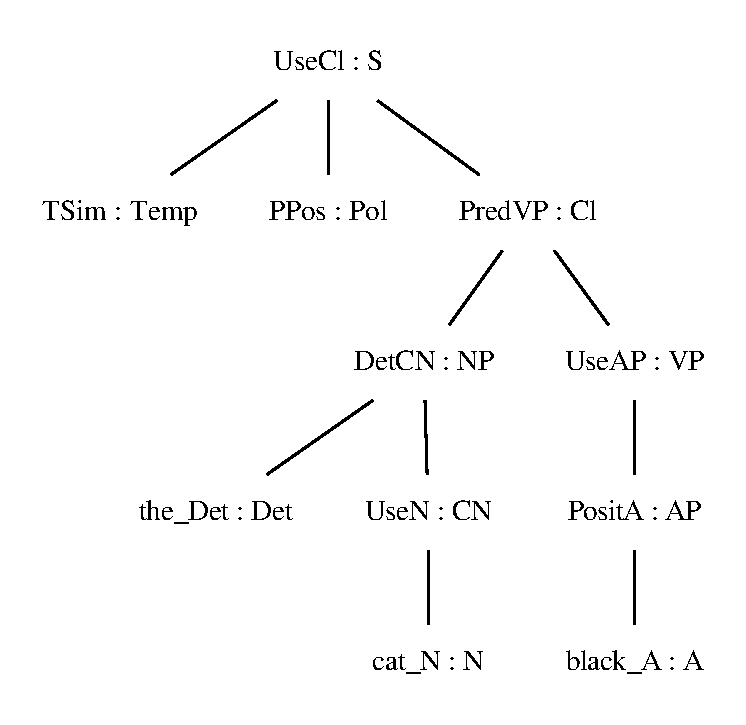
\includegraphics[width=0.5\linewidth]{figure/cat_is_black_gf.eps}
  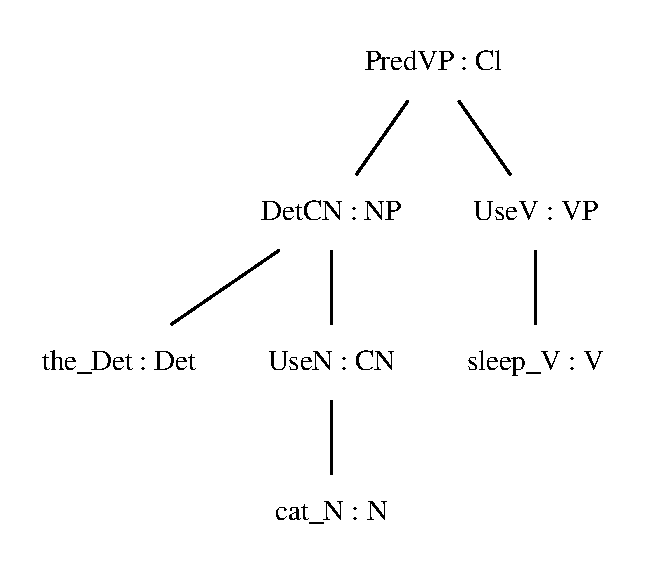
\includegraphics[width=0.5\linewidth]{figure/cat_sleeps_cl.eps}
  \caption{The sentence ``The cat sleeps'' analyzed as a GF tree}
  \label{fig:cat_sleeps_gf}
\end{figure}


% NOTES:
% "The cat is black" vs "The cat is not black" corresponds to PPos vs PNeg
% ud2gf would have trouble differentiating between these because it's only in parameters
% Macros UseCl_NegCop and UseCl_Sim corresponds to the different versions
% These allows the information to be preserved, despite there not being any explicit GF function for the word ``not''
%
% Negative:
% UseCl_NegCop (StrNeg "not") (PredVP (DetCN_theSg (StrThe "the") (UseN cat_N)) (UseAP_Cop (StrCop "be") (PositA black_A)))
% Positive:
% UseCl_Sim (PredVP (DetCN_theSg (StrThe "the") (UseN cat_N)) (UseAP_Cop (StrCop "be") (PositA black_A)))

% #auxfun UseCl_Sim cl : Cl -> S = UseCl TSim PPos cl ; head
% #auxfun UseCl_Ant have cl : Have -> Cl -> S = UseCl TAnt PPos cl ; aux head
% #auxfun UseCl_NegSim do neg cl : Do -> Neg -> Cl -> S = UseCl TSim PNeg cl ; aux advmod head
% #auxfun UseCl_NegAnt have neg cl : Have -> Neg -> Cl -> S = UseCl TAnt PNeg cl ; aux advmod head
% #auxfun UseCl_NegCop neg cl : Neg -> Cl -> S = UseCl TSim PNeg cl ; advmod head

% #auxfun UseAP_Cop cop comp : Cop -> AP -> VP = UseAP comp ; cop head

% #auxcat Cop AUX
% #auxcat Do AUX
% #auxcat Have AUX
% #auxcat Neg PART

% Syncategorematic words:
% #word not not Polarity=Neg
% #word does  do  Mood=Ind|Number=Sing|Person=3|Tense=Pres|VerbForm=Fin
% #word is   be  Mood=Ind|Number=Sing|Person=3|Tense=Pres|VerbForm=Fin
% #word would would  VerbForm=Fin
% #word will  will VerbForm=Fin

% Syncategorematic lemmas:
% #lemma UseCl,UseQCl,ImpVP not Neg advmod head
% #lemma UseAP,UseAdv,UseNP be Cop cop head
% #lemma PredVP have Have aux head
% #lemma PredVP,ImpVP do Do aux head

%  - strengths and weaknesses
%
\section{Differences between GF and UD}
% Strengths and weaknesses


% % Grammatical Framework has [some] advantages for [use-case], so it would be useful to be able to parse using UD and then get out a GF tree. A
GF is very strict when it comes to following grammar and spelling, which means that it will often refuse to parse sentences if they contain even the smallest error. UD on the other hand uses machine-learning to give some parse tree for all sentences regardless of how many errors they have.

While the machine-learning-based approach of UD allows it to guess the correct tree better for ambiguous sentences and allows it to handle grammatically incorrect sentences better, GF is much more capable when
it comes to performing transformations on the sentences, while maintaining correct morphology and grammar. This makes it attractive to parse sentences
using UD and then convert the parsed trees to GF trees in order to perform further transformations.


% Anteckningar

% UD har en massa manuellt annoterade träd som folk har tränat maskininlärningssystem på

% GF är mer strikt och kräver att grammatiken följs exakt och stavfel och små grammatikfel kommer inte

% UD är mer robust för fel och kommer alltid ge resultat oavsett om saker inte följs exakt och ger sin bästa gissning

% GF är mer exakt och förutsägbar, så buggar går bättre att anylysera och fixa

% Med GF kan man transformera meningar och träd på mycket fler sätt, till exempel kan ett påstående göras till en fråga bara genom att wrappa hela meningen med en MkQuestion funktion och då kommer automatiskt GF fixa alla morfosyntaktiska ändringar, så som att ändra ordföljd eller

% använder automatiskt rätt genus om man byter ut ett ord till ett annat

% abstrakt träd är oberoende av språk

% RGL beskriver morfosyntax för språk medan en applikationsgrammatik kan vara på högre nivå och ge mer ideomatiska översättningar och det beskrivs i termer av den abstrakta syntaxen för resursgrammatiken



% % Maybe mention the macros in the labels files

% % There exists a naive implementation based on a brute-force algorithm \cite{kolachina-ranta-2017}

% % Briefly describe and motivate the project, and convince the reader of the importance of the proposed thesis work.
% % A good introduction will answer these questions: Why is addressing these challenges significant for gaining new knowledge
% % in the studied domain? How and where can this new knowledge be applied?


\subsection{Useful synthesis between UD and GF}

% \todo[inline]{explain about gf-ud, the old-old version, the new-old version and my developments on that}

Prior to this work there existed a proof-of-concept implementation of a tool for converting between the trees for GF and UD,
with the help of so-called labels-files containing annotations which describe the mapping between UD labels and GF functions,
called gf-ud, which contains both a component for converting from UD to GF, called ud2gf\cite{kolachina-ranta-2017}\footnotemark[1]
and a component for converting from GF to UD, called gf2ud\cite{kolachina-ranta-2016}\footnotemark[1]. This work will focus on the ud2gf component.

\footnotetext[1]{These references apply to an older version of gf-ud, from before the one this thesis is based on. A part of the goal of this thesis is to document the later version in addition to documenting the changes made in the process of this thesis.}

% \todo{these references apply to an older version of gf-ud, from before the one I was working on. a part of the goal of this thesis is to document the old-new version that my changes was based on}

% The labels files can also contain macros, which allows constructing virtual GF functions during the translation from UD, which will be expanded to real GF functions at the end of the translation.
% These can, among other uses, be used to preserve information from the UD labels about subtrees, which can then be used at later points of the transformation to ensure that the desired GF tree is produced.

\subsection{Applications for the synthesis of UD and GF}

The gf-ud tool has been used for both translation and semantics\cite{ranta-al-2020}. %\todo{actually explain this}
Another application has been in concept alignment\cite{masciolini-ranta-2021}.
It has also been used to analyze legal texts as a part of a Controlled Natural Language for law\cite{listenmaa-etal-2021-towards}.

\section{What problem does ud2gf solve?}
% \todo[inline]{This is the main focus of the intro}
%
% \todo[inline]{Add edge labels to graph}
%
% \todo[inline]{write this text}

One problem within \ac{NLP} is converting from text to logic. There are several different paths one could take, each with their own issues, see \autoref{fig:text-to-logic} for an overview. The tool gf2ud makes it possible to get the robust parsing available for dependency trees and the ease of conversion to logic of Abstract Syntax Trees.

\begin{figure}[H]
    \centering
    % \includegraphics{}
    % \missingfigure{Graph of possible ways to convert from text to logic}
    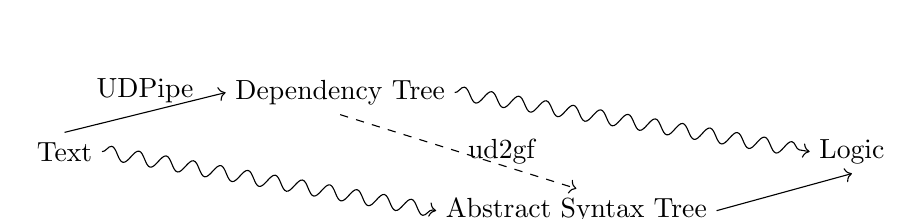
\begin{tikzpicture}
        \tikzset{snake it/.style={decorate, decoration=snake}}
		\node(Text) at (-5, 0) {Text};
		\node(DT) at (-1.5, 0.75) {Dependency Tree};
		\node(AST) at (1.5, -0.75) {Abstract Syntax Tree};
		\node(Logic) at (5, 0) {Logic};
		\draw[->] (Text.north) to node[above] {UDPipe} (DT.west);
		\draw[->, snake it] (Text.east) to (AST.west);
		\draw[->] (AST.east) to (Logic.south);
		\draw[->, snake it] (DT.east) to (Logic.west);
		\draw[->,dashed] (DT.south) to node[right] {ud2gf} (AST.north) ;
    \end{tikzpicture}
    \caption{An overview of how gf2ud can be helpful in converting from text to logic}
    \label{fig:text-to-logic}
\end{figure}

Converting from text to dependency trees is a solved problem\cite{Nivre2006,straka-etal-2016-udpipe,kanerva-etal-2020-turku}. Converting from AST to logic is a solved problem\cite{Montague1973-MONTPT-4,ranta-2004b,ranta2022end}. Converting from dependency trees to logic is a difficult problem\cite{reddy2016transforming,ranta2017explainable}. Converting from natural language text directly to AST is a difficult problem\cite{ranta-2011c,bernardy-stergios-2017,landin-1966-next-700,curry1961some,Montague1973-MONTPT-4}. By converting from DT to AST ud2gf allows us to use the two solved problems to get a path from text to logic.


% Från mallen


% This chapter presents the section levels that can be used in the template.
%
% \section{Section levels}
% \autoref{tab:sections} presents an overview of the section levels that are used in this document. The number of levels that are numbered and included in the table of contents is set in the settings file \texttt{Settings.tex}. The levels are shown in Section \ref{Section_ref}.
%
% This is a new paragraph and should have proper parskip or indentation. Don't forget to cite your sources~\cite{listenmaa-etal-2021-towards}. % '~' becomes space which cannot line break.
%
% \begin{table}[h]
% \centering
% \caption{Section levels} % Table text above table.
% \begin{tabular}{ll} \hline
% Name & Command\\ \hline
% Chapter & \textbackslash\texttt{chapter\{\emph{Chapter name}\}}\\
% Section & \textbackslash\texttt{section\{\emph{Section name}\}}\\
% Subsection & \textbackslash\texttt{subsection\{\emph{Subsection name}\}}\\
% Subsubsection & \textbackslash\texttt{subsubsection\{\emph{Subsubsection name}\}}\\
% %Paragraph & \textbackslash\texttt{paragraph\{\emph{Paragraph name}\}}\\
% %Subparagraph & \textbackslash\texttt{paragraph\{\emph{Subparagraph name}\}}\\ \hline\hline
% \end{tabular}
% \label{tab:sections}
% \end{table}

% \section{Section} \label{Section_ref}
% \subsection{Subsection}
% \subsubsection{Subsubsection}
% \paragraph{Paragraph}
% \subparagraph{Subparagraph}


% THEORY
% CREATED BY DAVID FRISK, 2016
\chapter{Theory}

In the following sections, examples of a figure, an equation, a table and a source code listing  are shown.

\section{Figure}
\begin{figure}[H]
\centering
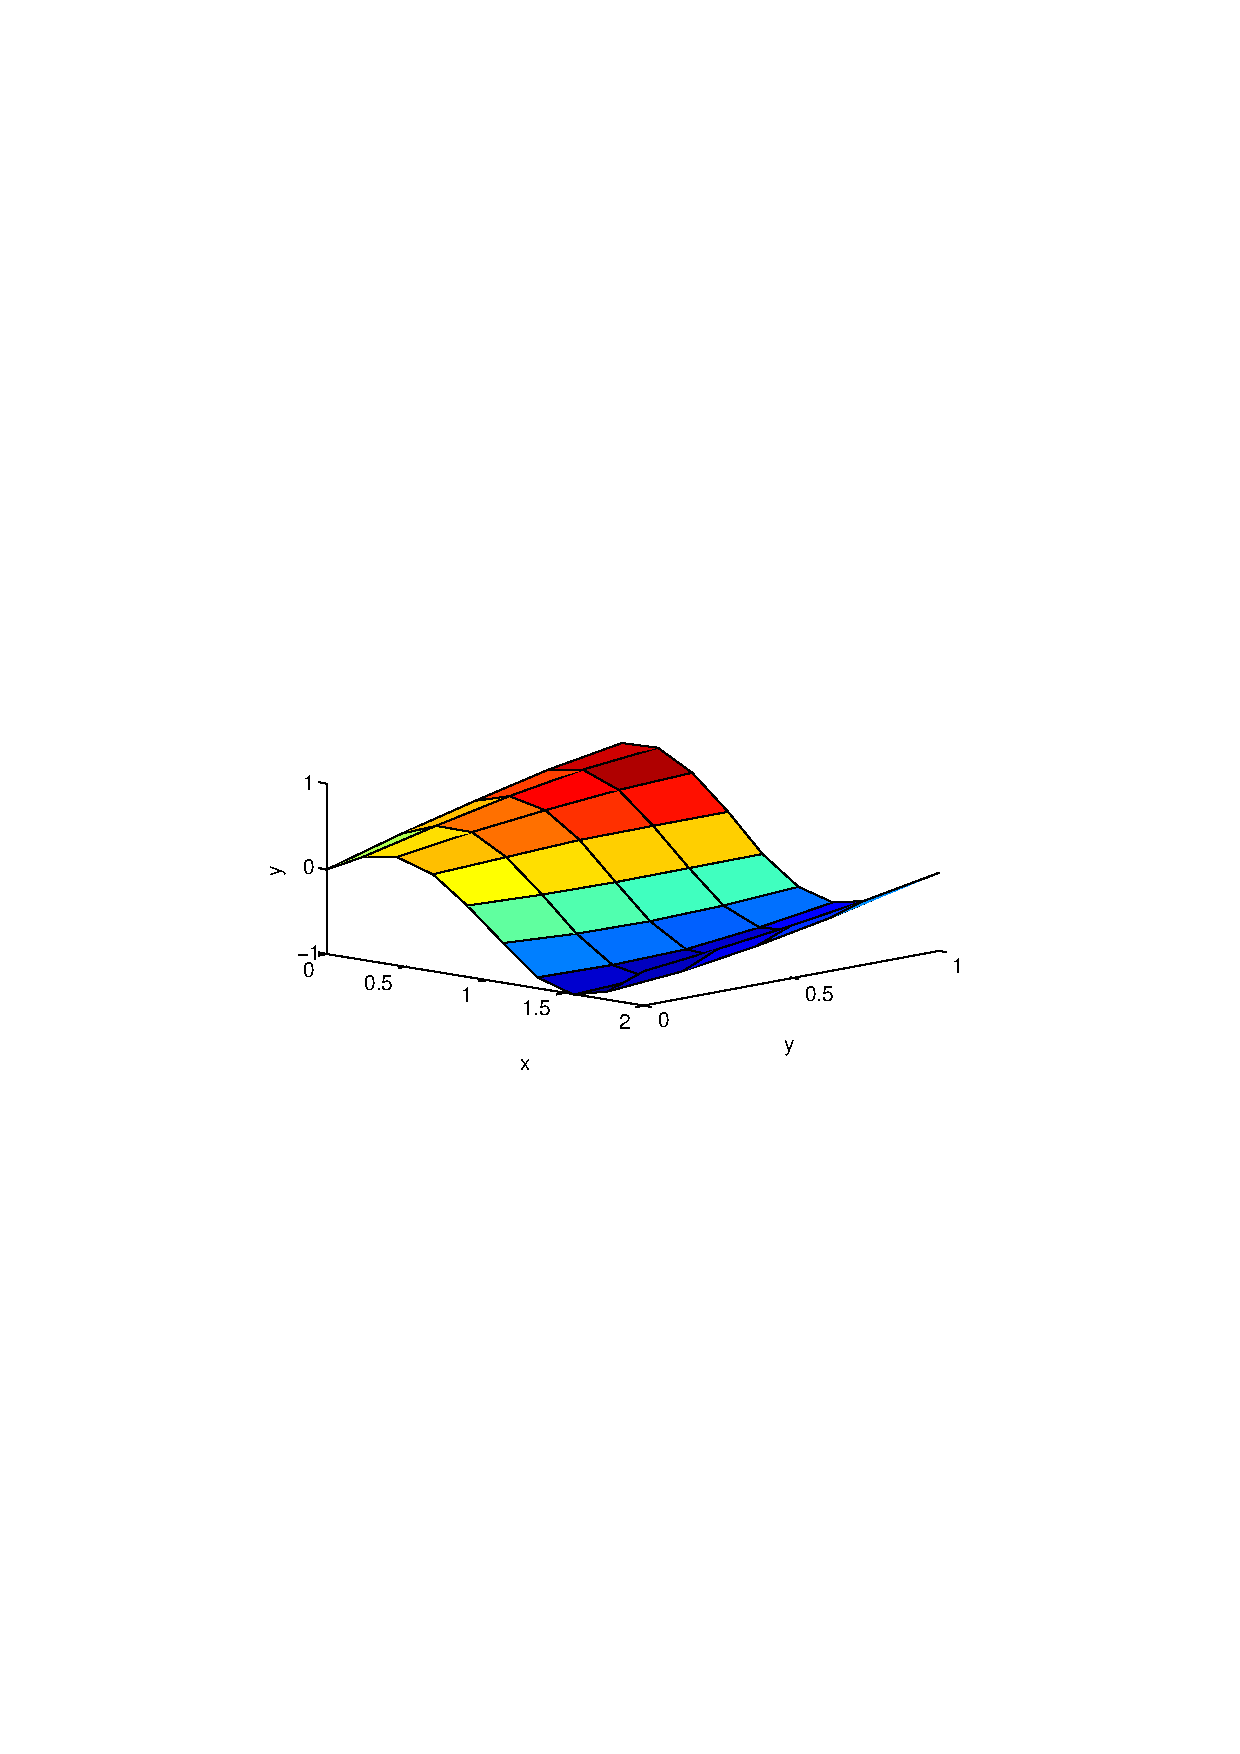
\includegraphics[width=0.45\linewidth, trim=3cm 11cm 3cm 11cm]{figure/X.pdf}
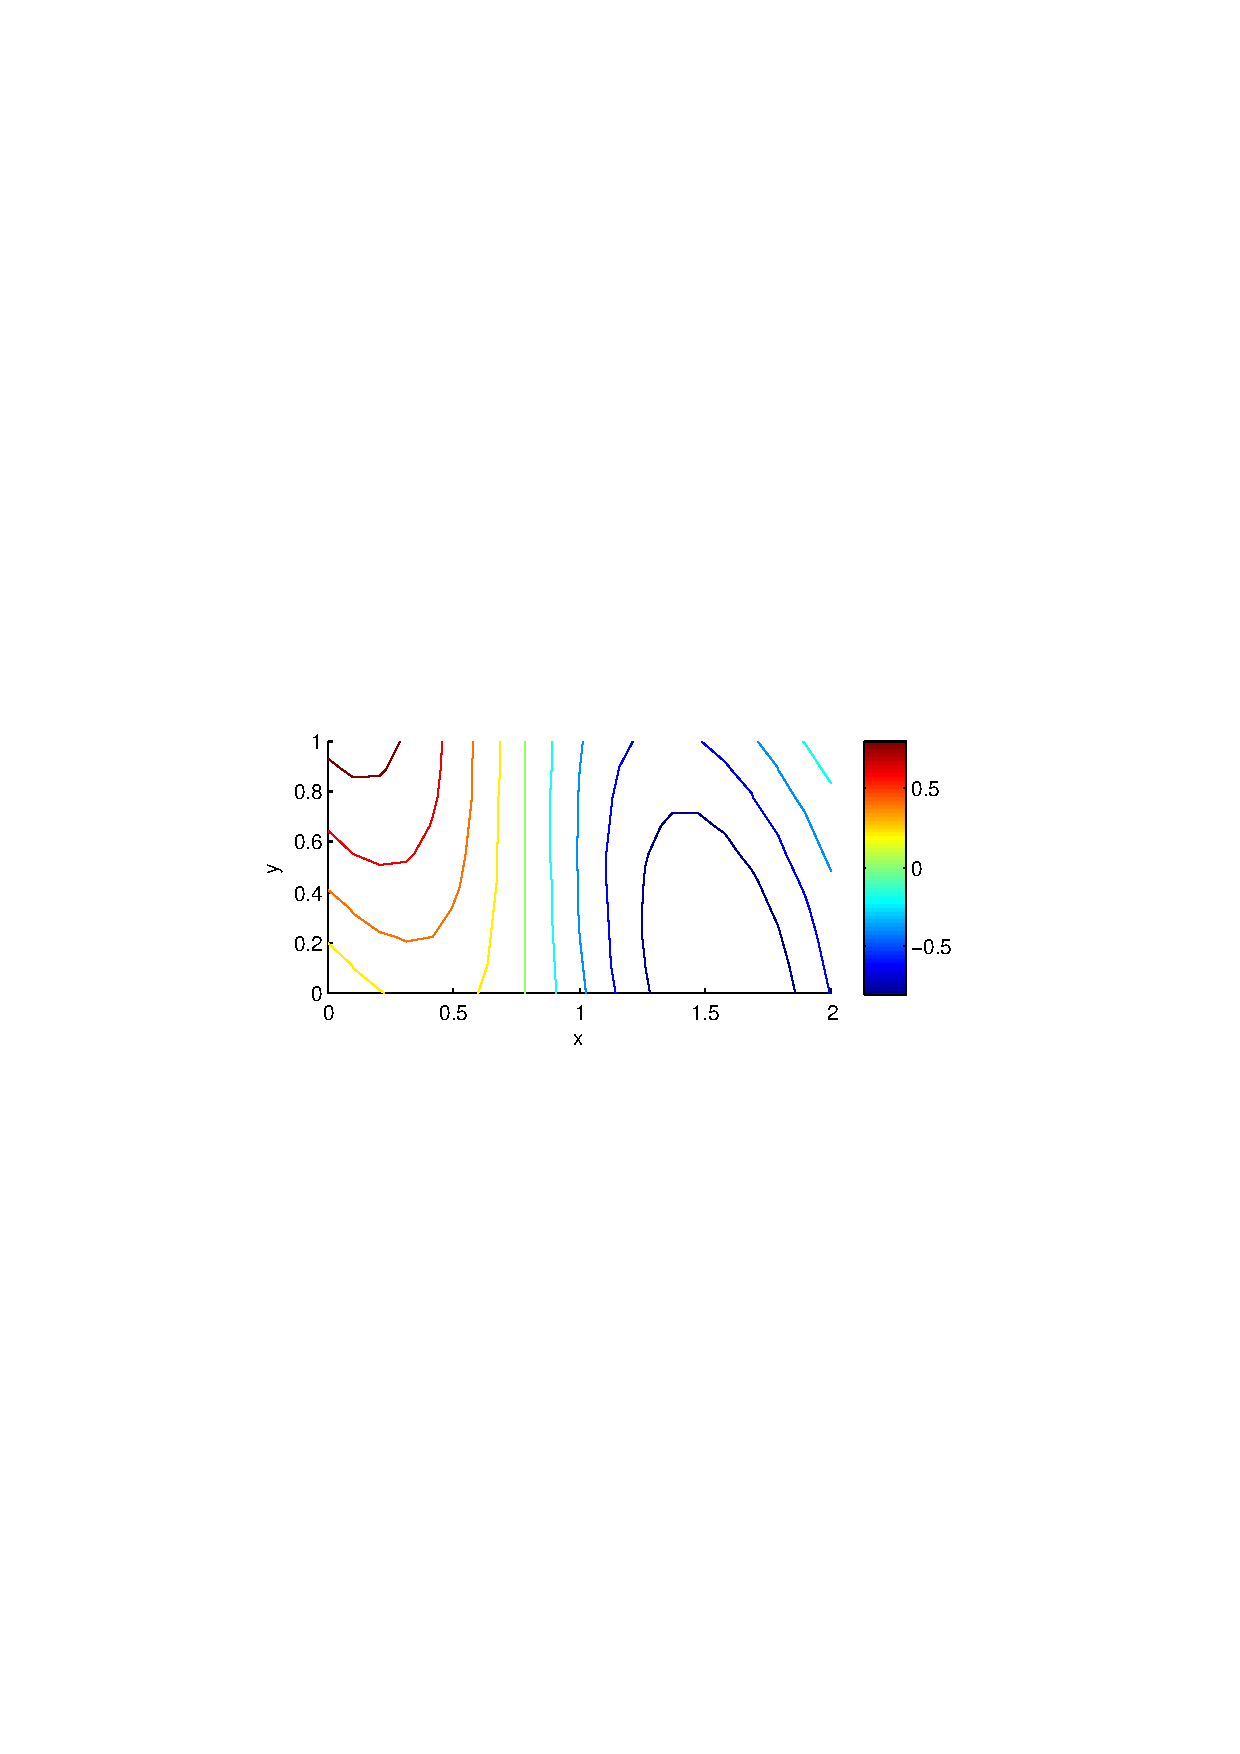
\includegraphics[width=0.45\linewidth, trim=3cm 11cm 3cm 11cm]{figure/Y.pdf}
\caption{Surface and contour plots showing the two dimensional function $z(x,y)=\sin(x+y)\cos(2x)$.} % Figure text below figure
\end{figure}

\section{Equation}
\begin{equation}
f(t)=\left\{ \begin{array}{ll}
1,~~~~ & t< 1 \\
t^2 & t\geq 1
\end{array}\right.
\end{equation}

\section{Table}
\begin{table}[H]
\centering
\caption{Values of $f(t)$ for $t=0,1,\dots 5$.}
\begin{tabular}{l|llllll} \hline\hline
$t$ & 0 & 1 & 2 & 3 & 4 & 5 \\ \hline
$f(t)$ & 1 & 1 & 4 & 9 & 16 & 25 \\ \hline\hline
\end{tabular}
\end{table}

\section{Chemical structure}
\begin{center}
\chemfig{X*5(-E-T-A-L-)}
\end{center}


\section{Source code listing}
\begin{minted}[frame=single]{matlab}
% Generate x- and y-nodes
x=linspace(0,1); y=linspace(0,1);

% Calculate z=f(x,y)
for i=1:length(x)
 for j=1:length(y)
  z(i,j)=x(i)+2*y(j);
 end
end
\end{minted}

\subsection{Other alternatives to the Theory chapter}
Sometimes, it is more appropriate to name this chapter Background.

At CSE, there exists a large span of different types of thesis works. Sometimes it is more appropriate to join the Theory and Methods chapters, sometimes the Theory chapter would be so small that it should be a subsection. Talk to your supervisor to find the most appropriate structure for your thesis.


\chapter{Background and Problem}

% - old ud-gf
% - newer naive approach - github + article 2017
%   - limitations
%   - performance


% Background to the assignment. Why is it relevant?
\section{Background}
\section{Problem}
% The formulation of the problem at hand and, the assignment. This should include an extended version of the scientific problem definition and references to knowledge within the area given in the thesis proposal.

% What has been done before and what remains to be done

% 2. Background & Problem
% - old ud-gf
% - newer naive approach - github + article 2017
%   - limitations
%   - performance

The current ud2gf implementation has some limitations. There are three main problems this work tries to fix.

The first problem is that it quickly becomes extremely slow for sentences with more than a couple of words and/or
when using large GF-grammars, e.g. GF-grammars containing Wordnet\cite{angelov2016predicting}. \\
The second problem is that if the structure differs too much between the representation of a sentence in UD format and as a GF tree, it is not possible to describe the required transformation in the current "labels file" language. See section \ref{sect:flex} below for more details. \\
The third problem is that it can sometimes be difficult to figure out why a rule in a labels-file is not firing, so it would be useful to have a debugging tool to help diagnosing such issues.


\subsection{Flexibility}\label{sect:flex}

As an example of a phrase that can be difficult to convert using the old gf2ud, let us consider the adjectival phrase "cute, fluffy and furry"
would be described in UD format as in Figures \ref{fig:ud_cute_text} and \ref{fig:ud_cute}.


\begin{figure}
    \begin{verbatim}
    1  cute  cute  ADJ  JJ  Degree=Pos  0  root  _  FUN=cute_A
    2  ,  ,  PUNCT  ,  _  3  punct  _  _
    3  fluffy  fluffy  ADJ  JJ  Degree=Pos  1  conj  _  FUN=fluffy_A
    4  and  and  CCONJ  CC  _  5  cc  _  FUN=and_Conj
    5  furry  furry  ADJ  JJ  Degree=Pos  1  conj  _  FUN=furry_A
    \end{verbatim}
    % \begin{tabular}{|c|c|c|c|c|c|c|c|c|c|}
    % \hline
    % 1 & cute & cute & ADJ & JJ & Degree\=Pos & 0 & root & \_ & FUN\=cute\_A \
    % \hline
    % 2 & , & , & PUNCT & , & \_ & 3 & punct & \_ & \_ \
    % \hline
    % 3 & fluffy & fluffy & ADJ & JJ & Degree\=Pos & 1 & conj & _ & FUN\=fluffy\_A \
    % \hline
    % 4 & and & and & CCONJ & CC & \_ & 5 & cc & \_ & FUN\=and\_Conj \
    % \hline
    % 5 & furry & furry & ADJ & JJ & Degree\=Pos & 1 & conj & \_ & FUN\=furry\_A \
    % \hline
    % \end{tabular}
    \caption{The phrase "cute, fluffy and furry" as a textual UD tree}
    \label{fig:ud_cute_text}
\end{figure}

\begin{figure}
    \centering
    % \begin{dependency}
  \begin{deptext}[column sep=0.4cm]
      cute \& , \& fluffy \& and \& furry \\
    {\tt ADJ}\&{\tt PUNCT}\&{\tt ADJ}\&{\tt CCONJ}\&{\tt ADJ} \\
  \end{deptext}
  \depedge{2}{1}{punct}
  \depedge{0}{2}{conj}
  \depedge{4}{3}{cc}
  \depedge{0}{4}{conj}
\end{dependency} \\
    % \includesvg{ud-annotatrix-corpus.svg}
    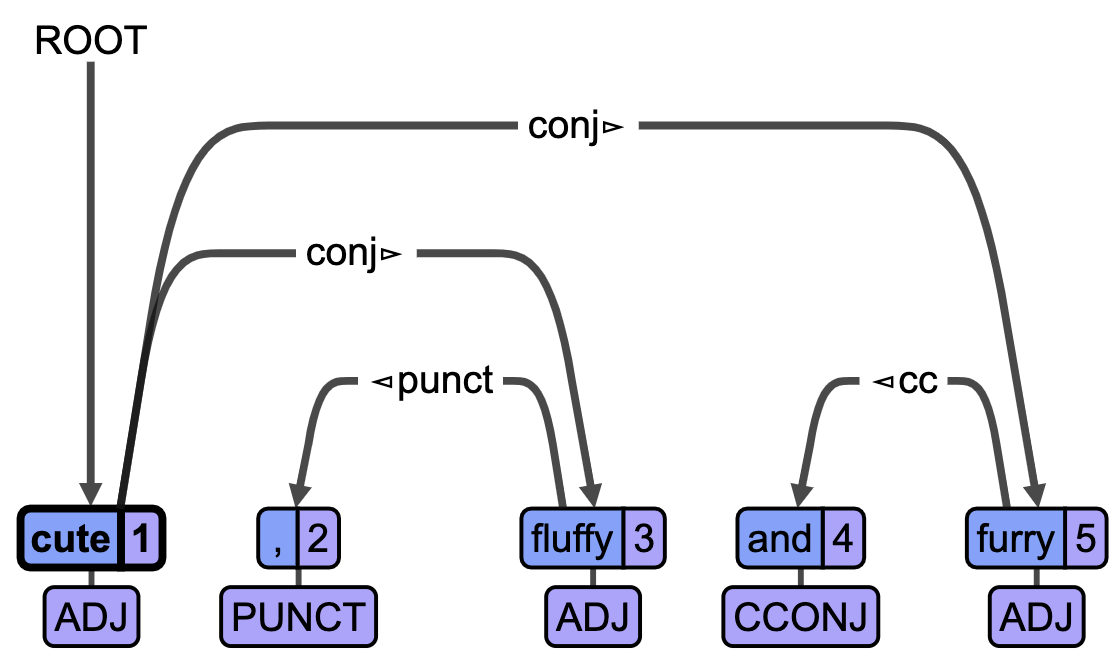
\includegraphics[width=0.7\textwidth]{figure/ud_cute.png}
    \caption{The phrase "cute, fluffy and furry" as a UD tree in graphical format}
    \label{fig:ud_cute}
\end{figure}
% \include{}

\begin{figure}
    \centering
    % \begin{dependency}
  \begin{deptext}[column sep=0.4cm]
      cute \& , \& fluffy \& and \& furry \\
    {\tt ADJ}\&{\tt PUNCT}\&{\tt ADJ}\&{\tt CCONJ}\&{\tt ADJ} \\
  \end{deptext}
  \depedge{2}{1}{punct}
  \depedge{0}{2}{conj}
  \depedge{4}{3}{cc}
  \depedge{0}{4}{conj}
\end{dependency} \\
    % \includesvg{ud-annotatrix-corpus.svg}
    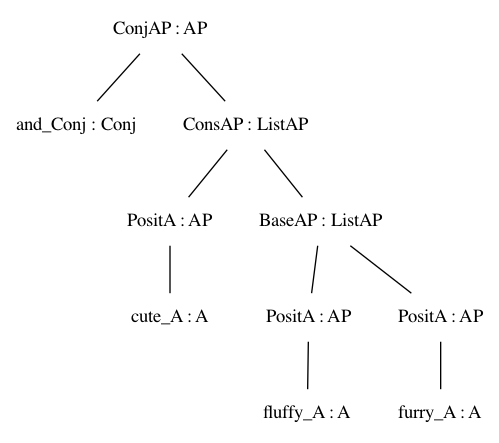
\includegraphics[width=0.7\textwidth]{figure/cute_gf.png}
    \caption{The phrase "cute, fluffy and furry" as a GF tree in graphical format. }
    \label{fig:gf_cute}
\end{figure}

The GF version of the same tree, shown in Figure \ref{fig:gf_cute}, would look like this:

\begin{verbatim}
ConjAP and_Conj (ConsAP (PositA cute_A)
                        (BaseAP (PositA fluffy_A) (PositA furry_A)))
\end{verbatim}
Here we can see that in UD, the word "cute" is in the root, while the conjunction "and" is at the bottom of the tree, while in GF the conjunction is a direct child of the root. This transformation can not be preformed by the simple single-layer transformations that are available in the current macro-system for labels files.

% Ideas:
%
% - Limits on how to transform trees - solution: extend language. currently hack using lambda calculus, but maybe better macros
%
% - Evaluate effectiveness of tool
%
% - (somewhere mention the performance boosts and analyse the complexity of it)

% This section is optional. It may be used if there is a need to describe the problem that you want to solve in more technical
% detail and if this problem description is too extensive to fit in the introduction.

% From elsewhere:
% - Background: GF \cite{ranta-2004}, UD \cite{nivre-etal-2016-universal},
%   - previous work: gf2ud \cite{kolachina-ranta-2016}, ud2gf \cite{kolachina-ranta-2017}
% - Describe the new algorithm
% - Extending the macro language
%   - Need for improvement: to match "fluffy and cute" needs 2 levels of nesting
%   - Solution: continuations
% - Case study: legal language

The translation described by a labels file is not one-to-one and there are often many possible GF trees that a UD tree could be translated to. The possible trees are currently ranked by completeness, as in how many of the words are included in the generated tree. However this ranking is incomplete and in case two possible trees, with the same GF category, cover the same words, an arbitrary tree will be chosen. A better choice could be to also check the linearization of these trees and rank those whose linearization is more similar to the original string higher. It would also be possible to completely exclude trees with differing linearization, but that would run counter to the goal of robustness.


% 3. The new algorithm
% - definitions
% - examples
% - how annotations work

% \section{Context}
% \todo[inline]{What's the difference between this and intro?}
% This work is mostly a continuation of the work in \cite{kolachina-ranta-2017}.

% A practical problem for which this tool can be useful can be found in \cite{listenmaa-etal-2021-towards}. In the Future Work section, under "Robust fall-back options", gf2ud is mentioned as a possible solution to making the parser more robust.

% % Use one or two relevant and high quality references for providing evidence from the literature that the proposed study indeed
% % includes scientific and engineering challenges, or is related to existing ones. Convince the reader that the problem addressed
% % in this thesis has not been solved prior to this project.

% Aim for the work. What should be accomplished?
\section{Goals and Challenges}

% try to preserve as much information as possible from the UD tree

% do this in an efficient way

% \todo[inline]{No longer relevant for final report?}

% \todo[inline]{Change this so it's clear that it has already been done}

1. Analyze algorithms and improve performance. The main challenge here is to find an algorithm for finding matching trees without exponential complexity on the number of children of a node in the UD tree.

2. Improve flexibility of macro language, allowing changing the structure of the trees while translating from GF to UD. One challenge here is in figuring out either how to change the algorithms to support these more advanced transformations or to find a way to allow them without needing to change the algorithms.

3. Write a debugging tool, which analyzes exactly what it is that prevents a rule in a labels-file from firing or what prevents that tree from being selected.
One challenge here is how to explain to the user the issue for all the possible things that can go wrong.
There is also an engineering challenge in making an algorithm that figures out what went wrong and why.
% either repeating the steps of the algorithm in order to find the issues or transforming the algorithm in a way that they can explain what went wrong

4. Document the version of the tool on which this work is based on, which had changed since what was written in \cite{kolachina-ranta-2017}


\subsection{Future work}

5. If there is time, update the algorithm to look at the linearization in order to try to select trees that match the original string as closely as possible and evaluate what difference this makes. This is only possible with improved performance from goal 1, but keeping it fast will still be a challenge. There are also some challenges here in how it should interact with the advanced macros in goal 2. We also need to handle when a GF tree has multiple linearizations, e.g. if it results in a conjugation table.

% % improve

% % Analyse the complexity of old and new algorithm, evaluate effectiveness of ...

% % Describe your contribution with respect to concepts, theory and technical goals. Ensure that the scientific and engineering
% % challenges stand out so that the reader can easily recognize that you are planning to solve an advanced problem.


% Limitations. What should be left out and why?
\section{Limitations}

Only the direction of converting UD trees to GF trees is studied here, because that is what was relevant to the application at hand. Furthermore, the two directions are almost completely independent in the implementation.

% I normalfallet behöver avgränsningarna inte motiveras.

% Limit the work mostly to what has already been done

% Har gjort:
%

%  \todo{why?}

% \todo[inline]{other limitations?}


\chapter{The new algorithm}
- definitions
- examples
- how annotations work

% METHODS
% CREATED BY DAVID FRISK, 2016
\chapter{Methods}
Methods text.



\section{Approach}
% Method of accomplishment. How should the work be carried out?

These methods were used for the different parts of the project

% \todo[inline]{Change these to past tense}
\subsection{Performance}

1. Finding the main source of slowness, which was done with profiling.

2. Analysing the current algorithms, which are based on brute force, trying all combinations, with some simple filtering.

3. Finding a better algorithm, which avoids exploring paths that could never be the correct answer and which avoids duplicate work.

4. Analysing the algorithmic complexity of both the new and the old algorithm and testing the practical performance to confirm the results.

\subsection{Flexibility}

In order to allow changing the shape of trees when translating from UD to GF, the macro language needs to be expanded.
A first prototype of this with minimal code changes has been done by making macro expansion recursive and then representing the code for the transformation in Church-encoding, inspired by lambda-calculus.

This approach can be evaluated by seeing how well it covers different tree shape changes for different trees one would encounter.

It could also be worthwhile to make a more user-friendly version of the advanced macros that can be understood without knowing about Church-encoding

\subsection{Debugging tool}
Going through each component of the algorithms in order to find where applying a rule can go wrong and add detection for them. Additionally trying out the debugging tool on a real grammar, e.g. in the context of \cite{listenmaa-etal-2021-towards}, in order to find edge-cases which were not handled by the debugging tool.

% Trial and error, whenever a problem arises that the tool doesn't find a helpful explanation for, try to add support for it.

\subsection{Linearization-aware translation}
Here we need a way to determine which linearization is actually closer and when to keep multiple options for a later stage of the translation. Some care also needs to be taken in determining which trees can be discarded and which ones need to remain available for a later stage.

Evaluating if the results are better with this version can be done in a large part by comparing the input string with the resulting string after translating to GF and linearizing.


% RESULTS
\chapter{Evaluation}
- synthetic experiment: RGL -> UD -> RGL
  - completeness - kan alltid få ett fullständigt träd
  - accuracy
  - performance
  - error analysis

% CREATED BY DAVID FRISK, 2016
\chapter{Results}
% Describe you results. Use tables, diagrams etc. for illustration.

\section{Performance}

% Undersök varför inte alla meningar ger samma resultat
% Kör hela upto12eng och jämför diff för statistik och hitta mönster

% Idé: Scatter-plot av optimerad mot ooptimerad

The result of running different versions of the algorithm on the example file \texttt{upto12eng.conllu} using the example grammar \texttt{ShallowParse} in the gf-ud git repository can be seen in \autoref{fig:time-including-gc}. The full list of sentences included in the benchmark can be seen in \autoref{app:upto12}. All benchmarks were perfomed on a 2019 MacBook Pro, with a 2.3 GHz 8-Core Intel Core i9 CPU.

\begin{table}[]
    \centering
    \begin{tabular}{c|ccc}
Time (seconds) & Calculation & Garbage Collection & Total \\
\hline
Original code & 2m 58s 834ms & 24s 637ms & 3m 23s 471ms \\
Original code (fast GC) & 3m 1s 872ms & 20s 241ms & 3m 22s 113ms \\
fastKeepTrying & 26s 171ms & 14s 767ms & 40s 938ms \\
fastKeepTrying (fast GC) & 28s 631ms & 1s 705ms & 30s 336ms \\
fastAllFunsLocal & 3s 166ms & 14s 31ms & 17s 197ms \\
fastAllFunsLocal (fast GC) & 3s 203ms & 1s 253ms & 4s 456ms \\
Both improvements & 2s 687ms & 13s 922ms & 16s 609ms \\
Both improvements (fast GC) & 1s 253ms & 1s 253ms & 2s 506ms \\
    \end{tabular}
    \caption{The total run time for converting the file upto12eng.conllu, including garbage collection and startup time. The bars marked ``fast GC'' have increased initial heap size to 500Mb to reduce the number of unnecessary garbage collections, based on the experiments in \autoref{sect:gc-time}. TODO: Perform multiple measurements to reduce noise. Also, don't include milliseconds, when we don't have that precision. }
    \label{tab:time-with-gc}
\end{table}

In \autoref{fig:time-vs-time} we can see the speedup for each individual sentence. The improvement of the keepTrying function gives a close to linear speedup, while the speedup from the optimized version of allFunsLocal is much larger. The theoretical expected speedup from keepTrying is a quadratic factor that becomes a linear factor based on the depth of the resulting trees. This 
\begin{figure}
    \centering
    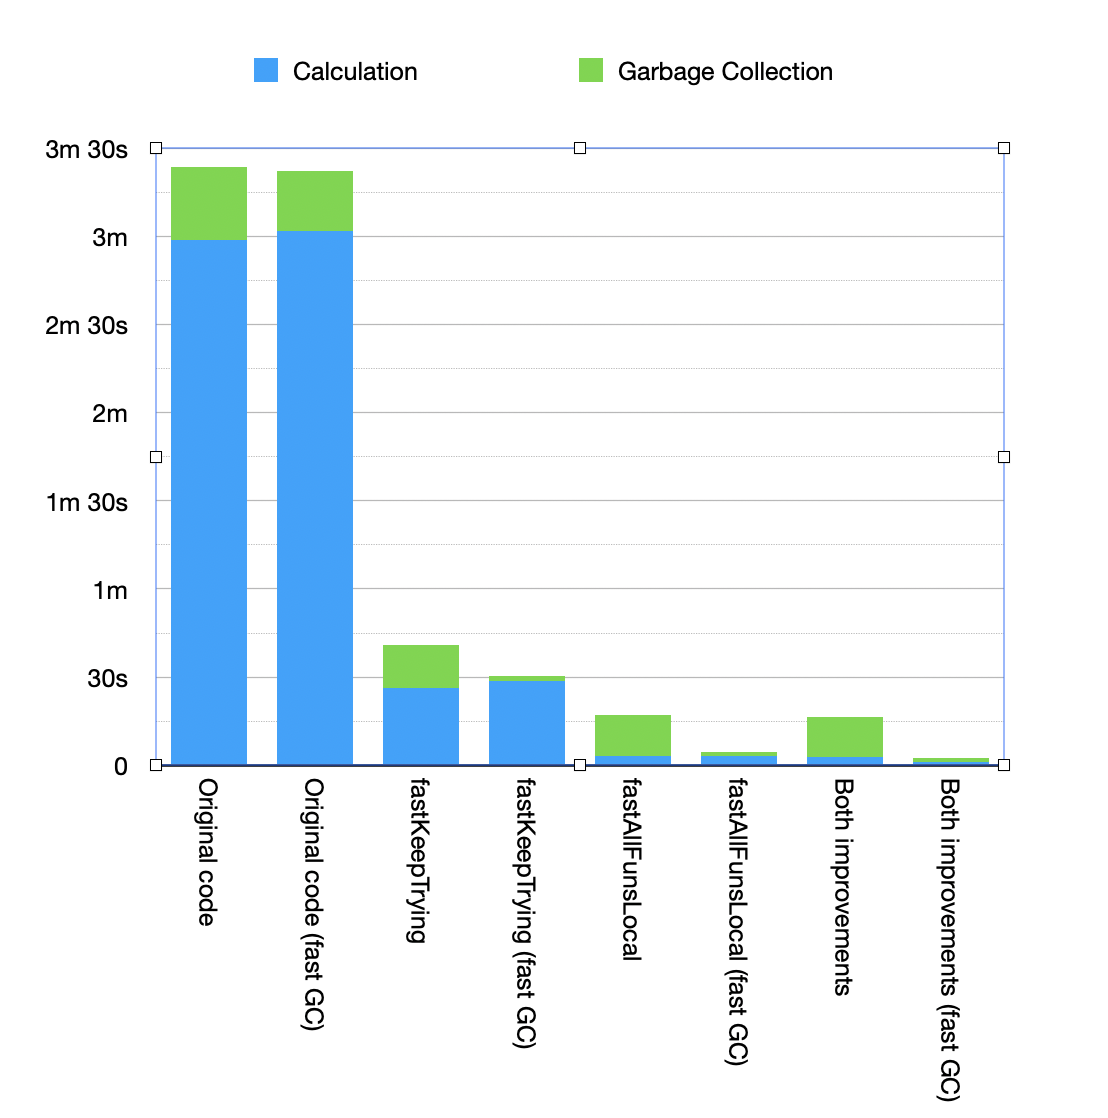
\includegraphics[scale=0.75]{thesis/figure/Time-including-GC.png}
    \caption{The total run time for converting the file upto12eng.conllu, including garbage collection and startup time. The bars marked ``fast GC'' have increased initial heap size to 500Mb to reduce the number of unnecessary garbage collections, based on the experiments in \autoref{sect:gc-time}. TODO: Perform multiple measurements to reduce noise.}
    \label{fig:time-including-gc}
\end{figure}

\begin{figure}
    \centering
    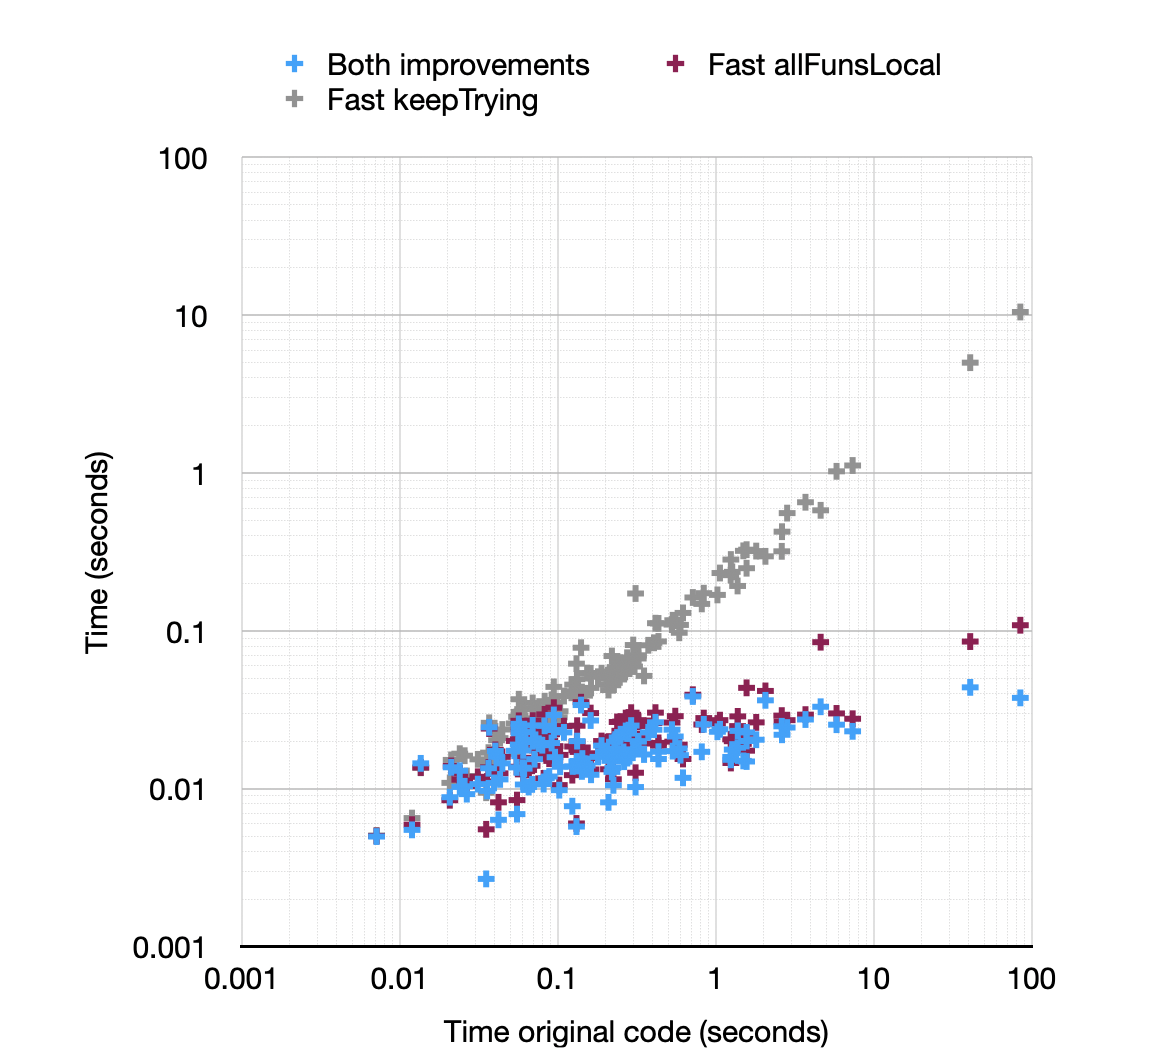
\includegraphics[scale=0.75]{thesis/figure/Time-against-time-plot.png}
    \caption{A log-log plot of time for each optimization against the time for the original algorithm. Each data point is the average time over several runs for a single sentence. The library Criterion\protect\footnotemark{} was used to perform the measurements.}
    \label{fig:time-vs-time}
\end{figure}

\footnotetext{http://www.serpentine.com/criterion/}

In \autoref{fig:keepTrying-speedup-factor} we can see that the speedup from the keepTrying improvement is linear with respect to the logarithm of the original code, which matches the expectation of moving from converting a quadratic factor to a linear factor. 
Looking at the slowest sentence ``In Danish, the word may even apply to shallow lagoons'', it takes 83 seconds with the original algorithm and 10 seconds with the keepTrying improvement, giving a speedup factor of 8.3. Looking at the generated tree we can confirm that it has a maximum tree depth of 9 at the top, matching the expectation.

\begin{figure}
    \centering
    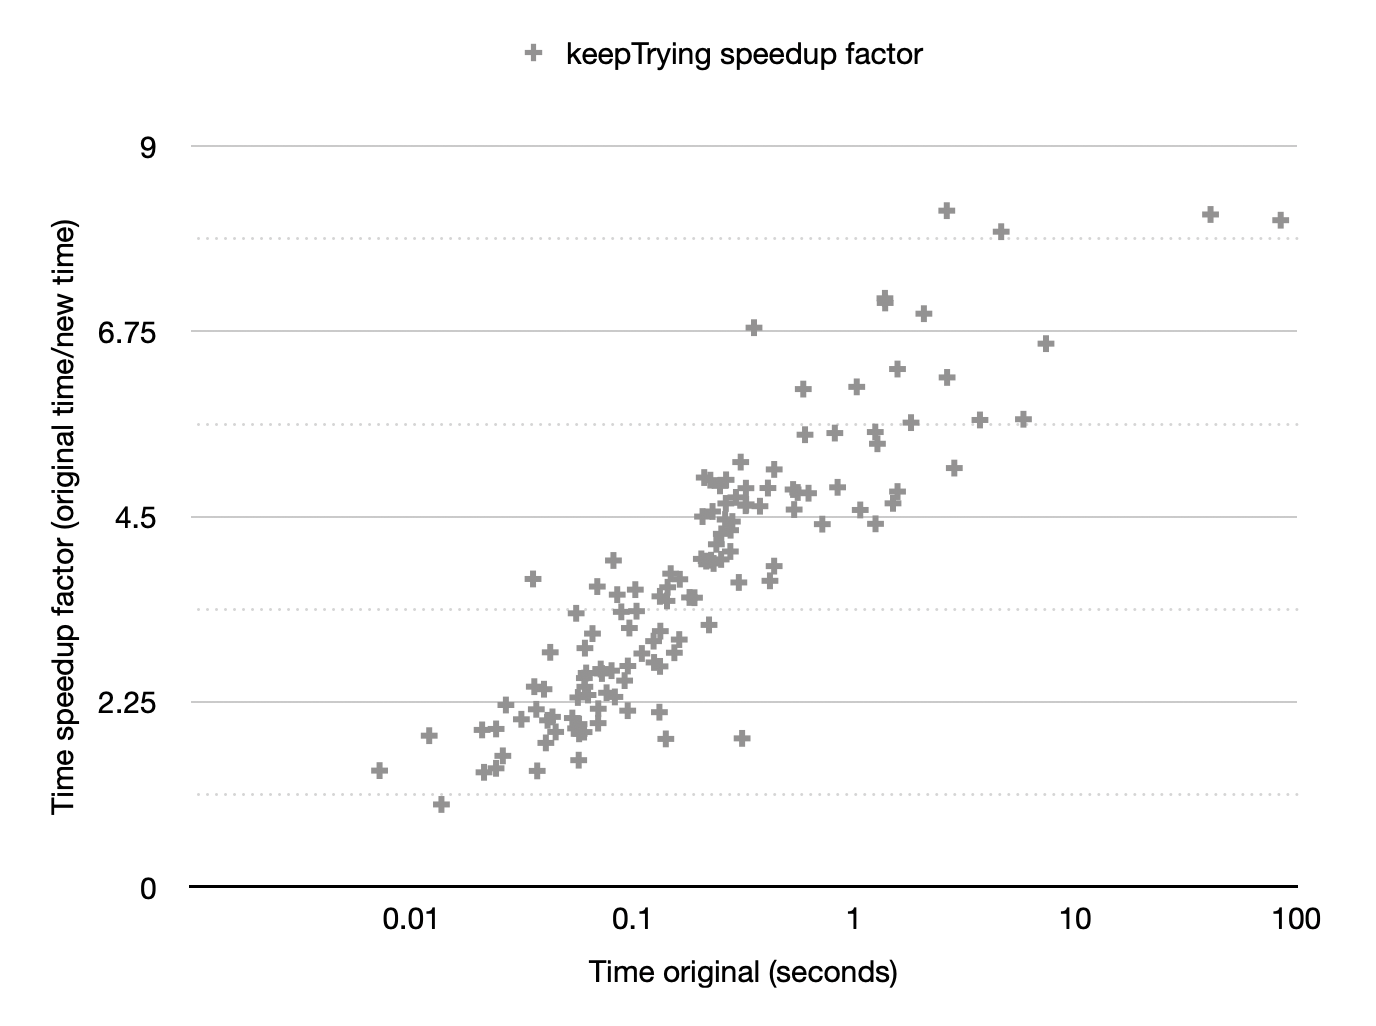
\includegraphics[scale=0.5]{thesis/figure/keepTrying-speedup-factor.png}
    \caption{A plot of the speedup factor for the improved keepTrying algorithm: new time divided by original time, against the original time taken. A linear speedup is the expected result for converting a quadratic algorithm to a linear algorithm.}
    \label{fig:keepTrying-speedup-factor}
\end{figure}

In \autoref{fig:allFunsLocal-speedup-factor} we can see that the allFunsLocal improvement has a speedup factor that is linear on the log-log plot, which indicates that we got an exponential speedup as expected from the theory.

\begin{figure}
    \centering
    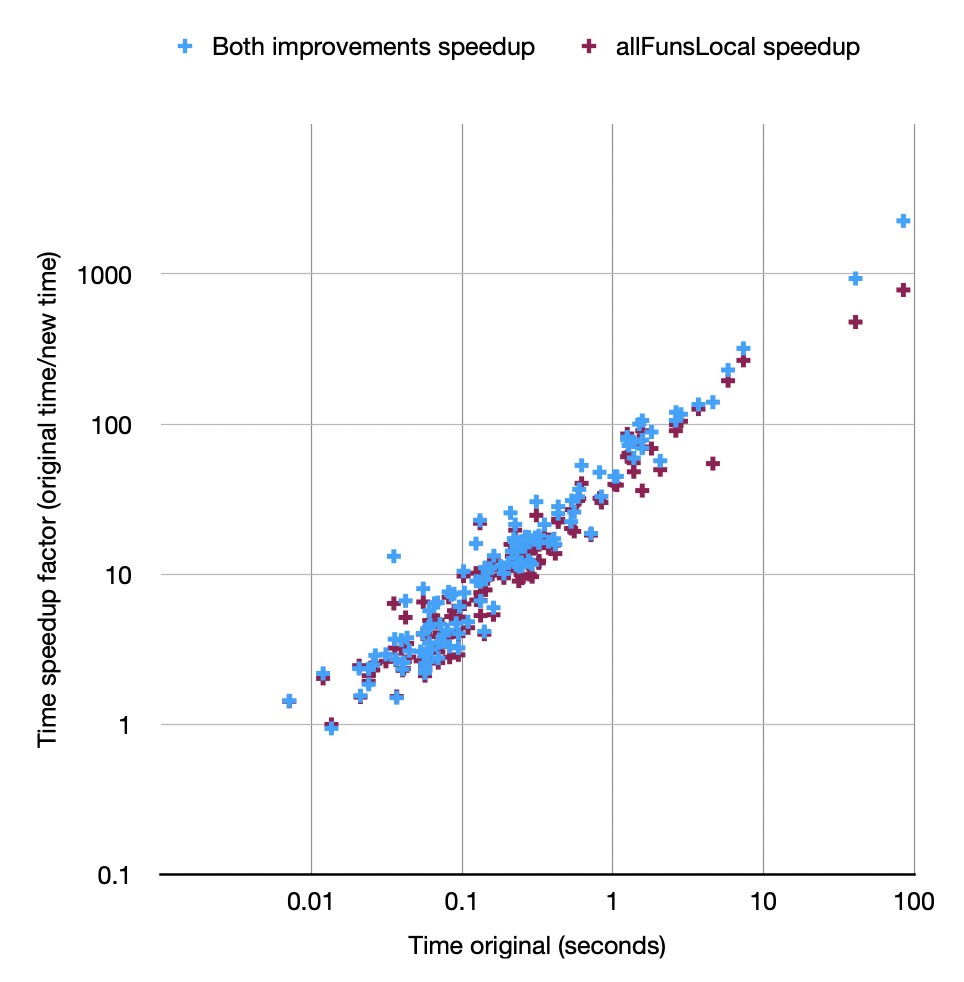
\includegraphics[scale=0.75]{thesis/figure/allFunsLocal-speedup-factor.png}
    \caption{A log-log plot of the speedup factor for the improved allFunsLocal algorithm: new time divided by original time, against the original time taken. The linear pattern indicates an exponential speedup.}
    \label{fig:allFunsLocal-speedup-factor}
\end{figure}

TODO: Write about the minor changes in the resulting trees from the optimized version of the keepTrying function.

% DONE: \todo[inline]{Stacked diagram of all four configurations, with GC time included}


% Running on upto12eng with both improvements and default Garbage Collection settings
% \begin{verbatim}
%    7,783,705,112 bytes allocated in the heap
%   13,905,705,592 bytes copied during GC
%      178,448,096 bytes maximum residency (37 sample(s))
%        2,051,952 bytes maximum slop
%              516 MiB total memory in use (0 MB lost due to fragmentation)
% 
%                                      Tot time (elapsed)  Avg pause  Max pause
%   Gen  0      7351 colls,     0 par    9.128s   9.260s     0.0013s    0.0056s
%   Gen  1        37 colls,     0 par    4.828s   5.069s     0.1370s    0.2165s
% 
%   INIT    time    0.000s  (  0.005s elapsed)
%   MUT     time    2.612s  (  2.666s elapsed)
%   GC      time   13.956s  ( 14.329s elapsed)
%   EXIT    time    0.000s  (  0.005s elapsed)
%   Total   time   16.569s  ( 17.004s elapsed)
% 
%   %GC     time       0.0%  (0.0% elapsed)
% 
%   Alloc rate    2,979,803,301 bytes per MUT second
% 
%   Productivity  15.8% of total user, 15.7% of total elapsed
% \end{verbatim}


\subsection{Garbage Collection time}\label{sect:gc-time}
As can be seen from the previous section, after the improved algorithm is used over 80\% of time is spent on garbage collection. This is in a large part because GHC uses a generational, moving garbage collector\cite{ungar1984generation}, which means that the cost of a garbage collection is proportional to the amount of currently living data \todo{Source for this claim}. In our case we have a large amount of long-living data, which means that every major garbage collection is expensive. The code begins by loading the GF grammar into memory, which for our test grammar takes up around 100 megabytes. There are several ways to mitigate this, but the easiest solution is to tweak the parameters for the garbage collector to make it wait longer before attempting to collect garbage, which reduces the total number of major garbage collections.


% \todo[inline]{The text above should probably go elsewhere (if anywhere at all)}

The tool ghc-gc-tool allows automatically determining which parameters are best for this by running the executable with different parameters and plotting the result. In \autoref{fig:gf-ud-integ-gc-space} we can see the result of running this on the first 60 items of upto12eng.conllu with the ShallowParse grammar from the repository. This number was chosen arbitrarily to make the runtime not be unreasonably long. 

As can be seen in \autoref{fig:GC-time} any initial heap size over 256M drastically reduces the run time and the logs show that the productivity (time spent on non-GC) goes from 15\% to 50\% and that less than one tenth as many garbage collections are performed. This number depends on the size of the GF grammar and it corresponds to the size of the GF grammar after being loaded into memory. Running the command with the default GC parameters shows that the maximum residency is 180M, which is slightly less than the optimal GC parameter value.

\begin{verbatim}
$ ghc-gc-tune -t pdf -spr gf-ud ud2gf grammars/ShallowParse Eng Text
...
gf-ud +RTS -A32768 -H134217728 -RTS ud2gf grammars/ShallowParse Eng Text
    <<GCs 125563, peak   538, resident 177.67m, MUT 1.728s, GC 9.609s>>
gf-ud +RTS -A32768 -H268435456 -RTS ud2gf grammars/ShallowParse Eng Text
    <<GCs   8655, peak   509, resident 176.64m, MUT 1.211s, GC 1.776s>>
...
\end{verbatim}

\begin{figure}
    \centering
    \subcaptionbox{Integral of space use over time\label{fig:GC-time-integ}}
      {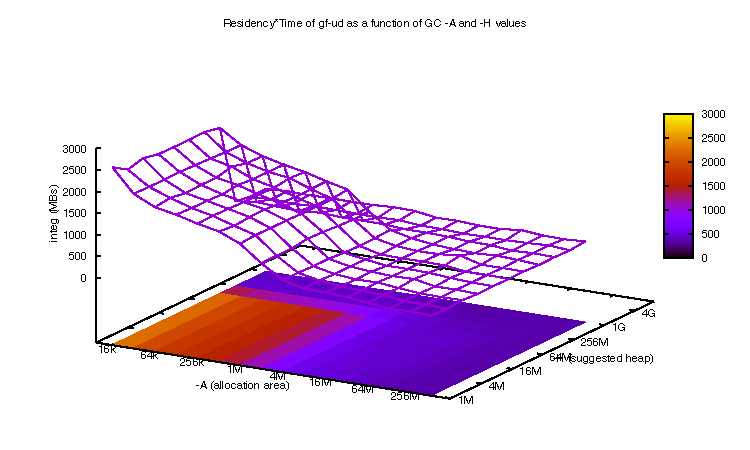
\includegraphics[scale=0.5]{thesis/figure/gf-ud-integ-gc-space.pdf}}
    \subcaptionbox{Time taken\label{fig:GC-time}}
      {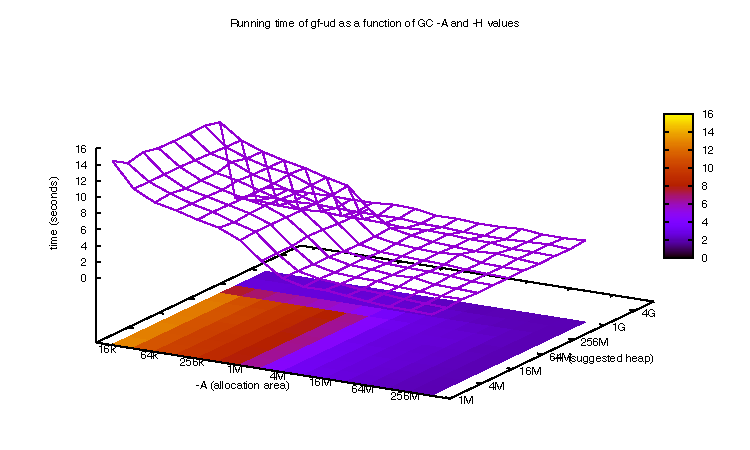
\includegraphics[scale=0.5]{thesis/figure/gf-ud-time-gc-space.pdf}}
    \subcaptionbox{Resident space usage\label{fig:GC-resident-space}}
      {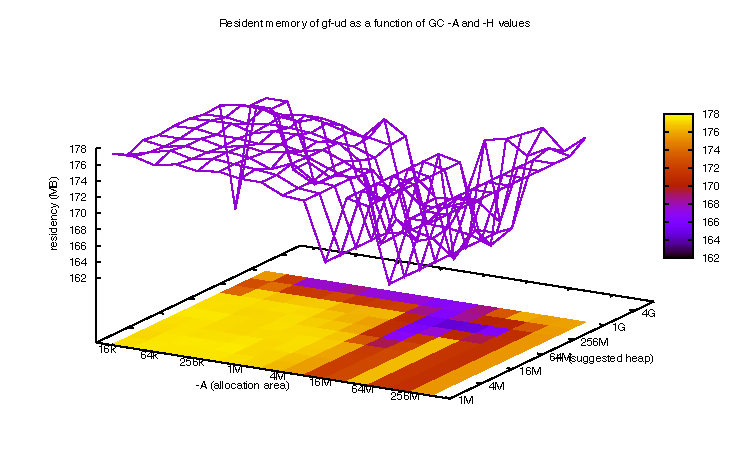
\includegraphics[scale=0.5]{thesis/figure/gf-ud-residency-gc-space.pdf}}
    \subcaptionbox{Peak space usage\label{fig:GC-peak-space}}
      {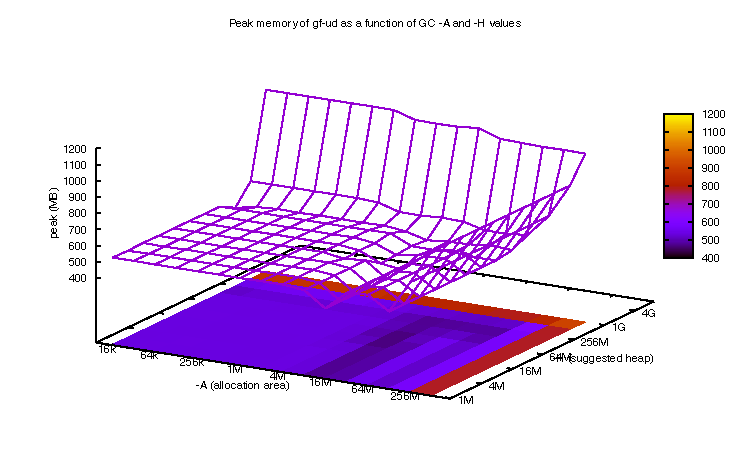
\includegraphics[scale=0.5]{thesis/figure/gf-ud-peak-gc-space.pdf}}
    \caption{The integral of space usage over time for different GC parameters}
    \label{fig:gf-ud-integ-gc-space}
\end{figure}

We also explored other methods for reducing the impact of garbage collection, like compact regions\cite{yang2015efficient}, but they provided no improvement over the simpler method of tweaking the GC parameters and in some cases using them made performance worse, because they force all data stored to be fully evaluated.

\section{Correctness}

Because the accuracy of the conversion depends on manually written annotation files, evaluating the accuracy of the conversion is outside of the scope for this paper.

The optimization of the \texttt{allFunsLocal} function had no impact on the generated trees. However, in some cases the optimization of the \texttt{keepTrying} functions caused different trees to be picked. The different trees are equally valid according to the defined constraints in the annotations and some of them are better and some are worse fits in the example trees we evaluated. See \autoref{sec:multiple_trees} for more details on the multiple possible trees.

\section{Debugging}

The debugging tool that was written in this project allows finding what prevented an \#auxfun macro from being used to convert a tree and anecdotal evidence points towards it being helpful when writing annotations.


\section{Flexibility}

%The new recursive macros made it possible to express the tree shape changes required to convert from the UD way of writing coordination into the GF way of writing conjunctions. Initial tests were successful in converting coordinate structures\footnote{For example ``furry, fluffy and cute'' or ``dog, cat or capybara''} of different lengths and different parts of speech. 

The new recursive macros made it possible to express more significant changes in tree shapes when converting between UD and GF. The motivating example is \emph{coordination}: structures like ``big \emph{or} small'' or ``cats, dogs \emph{and} capybaras''. Before the recursive macros, it was only possible to convert structures with exactly 2 conjuncts, since those had sufficiently similar structure, but now ud2gf can convert coordinate structures of arbitrary length.


\section{Use in robust parsing}

As mentioned in \autoref{sect:background}, the improvement of ud2gf was done as a part of the SMU CCLAW project, with the goal of using ud2gf as a part of a pipeline for parsing unrestricted text in the legal domain.
Experiments on that were performed on a small scale, but the results were deemed unsatisfactory for that specific use. A major part of the problem was the correctness of udpipe itself: legal text contains many uncommon structures, and the initial parses were inaccurate relatively often. 
Given the dissatisfaction with the approach, we never did a quantitative evaluation of the results.

Anecdotally, we found the macro system useful in recovering from parser errors, but it was a lot of tedious work\footnote{Example auxfuns written to recover from errors in udpipe output can be found at \url{https://github.com/smucclaw/sandbox/blob/default/inari/ud/copied-from-dsl/grammars/UDAppEng.labels\#L105-L136}}, with a long tail of fixes that only applied to a single sentence. 

% Write something about the results of using it in the singapore project

% Tie back to section 1.4

% Notes:
% Move info about the singapore project earilier in intro
%



% CONCLUSION
% CREATED BY DAVID FRISK, 2016
\chapter{Conclusion}

You may consider to instead divide this chapter into discussion of the results and a summary. 

\section{Discussion}

\section{Conclusion}


% REFERENCES / BIBLIOGRAPHY
\cleardoublepage
\phantomsection % So hyperref does not link to the section above
\addcontentsline{toc}{chapter}{Bibliography}
\printbibliography

% APPENDICES
\cleardoublepage
\appendix
\setcounter{page}{1}
\pagenumbering{Roman}			% Capitalized roman numbering starting from I (one)

% CREATED BY DAVID FRISK, 2016
\chapter{Appendix 1}




\end{document}
